% 4. Execution Framework and State Machine
% ----
\section{XF et Machines d'états}
Une machine d'état est composée d'un nombre fini :
\begin{enumerate}
    \item d'états, qui peuvent avoir des actions :
    \begin{enumerate}
        \item sur l'entrée
        \item continue
        \item sur la sortie
    \end{enumerate}
    \item de transistions :
    \begin{enumerate}
        \item déclenchée par un événement,
        \item peuvent avoir condition,
        \item et peuvent exécuter une action
    \end{enumerate}
    Ces éléments sont signalés via des décorateurs : \verb+trigger[guard]/action+
    
    Exemple :
    \begin{figure}[H]
    \centering
        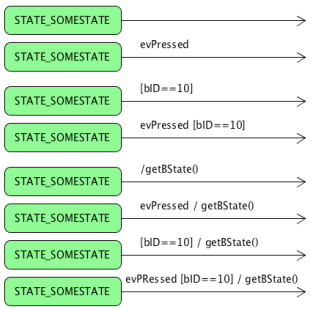
\includegraphics[width=4.00cm]{figures/state_trans.png}
\end{figure}
\end{enumerate}
% ----
\subsection{XF}
Le XF est une couche d'abstraction pour l'OS (interface seulement) ou offre des services similaires à un OS (interface + implémentation dans ce cas).

Opération atomique : opération garantie d'être exécutée sans interruptions ($\rightarrow$ une seule étape).

\subsection{ISI double switch SM pattern}
Machine d'état à double switch :
\begin{itemize}
    \item Un switch de transition
    \item Un switch d'action
\end{itemize}